\chapter{Desarrollo del sistema}
En este capítulo se explicarán las tecnologías utilizadas y las arquitecturas internas de cada subsistema. Los dos subsistemas que desarrollaremos
serán el HUB y la Interfaz.
\label{chap:desarrollosistema}
\lsection{Stack tecnológico}
Elegir el stack tecnológico a utilizar en el desarrollo de cualquier sistema es siempre una tarea difícil y determinante en el desarrollo de 
cualquier proyecto. Una elección inacertada puede significar el fracaso de un proyecto, mientras que una elección acertada sginificará que el 
proyecto salga adelante cumpliendo con todas las expectativas.
\par
Para elegir el stack correcto necesitamos tener en cuenta varios aspectos:
\begin{itemize}
\item\underline{Madurez de la tecnología:} es importante utilizar una tecnología con cierta madurez para evitar bugs, incompatibilidades, etc. Además, es
conveniente optar siempre por versiones LTS y evitar versiones Beta.
\item\underline{Comunidad/respaldo de la tecnología:} por lo general, este punto está muy relacionado con el punto anterior, ya que cuanta más madurez tiene
una tecnología, más comunidad suele existir. Aunque no sólo la madurez influye, si no la popularidad de la tecnología, cuanto más se use esa tecnología,
más comunidad tiene. La comunidad de una tecnología, junto con su documentación, ayudan al desarrollador a enfrentarse a los problemas que surgen a lo
largo del desarrollo, siendo capaces de ver o preguntar a otros desarrolladores que ya se hayan enfrentado a dicho problema.
\item\underline{Conocimiento de los desarrolladores:} este punto es esencial, ya que es necesario que el equipo de desarrollo conozca las tecnologías, o en caso
contrario, ser capaces de contratar nuevos desarrolladores que sí las conozcan. La popularidad de la tecnología es esencial en este punto, ya que, por 
lo general, es más sencillo encontrar desarrolladores que conozcan tecnologías populares.
\item\underline{Librerías externas:} junto a la comunidad, las librerías externas ayudan a los desarrolladores a solucionar problemas que ya han sido resueltos
por otros desarrolladores. Por ejemplo, librerías para el manejo de fechas, librerías para gestionar conexiones con bases de datos...etc.
\item\underline{Licencias/mantenimiento de la tecnología:} es necesario tener en cuenta las licencias y el mantenimiento de las tecnologías antes de elegirlas,
pues pueden suponer gastos bastante elevados.
\end{itemize}

Teniendo en cuenta los apartados anteriores, se ha optado por utilizar Express.js junto sqlite para el desarrollo del HUB, e Ionic para el desarollo de
la interfaz gráfica.

\begin{figure}[H]
\centering

\includegraphics[width=5.00in]{images/stack_tecnologico.png}
\caption{Stack tecnológico escogido}
\label{fig:stack_teconologico}
\end{figure}

\subsection{Express.js}
Se trata de un framework para Node.js enfocado en el desarrollo de aplicaciones web. Utiliza JavaScript como lenguaje principal, un lenguaje moderno, muy popular y
muy rápido en ejecución. Los desarrolladores de express definen a su framework como: \textit{``Infraestructura web rápida, minimalista, y flexible para Node.js``}.
Además, según \textbf{hackr.io}: \textit{``Express es uno de los frameworks que más rapido está creciendo en popularidad, y es utilizado por compañías como Accenture, IBM o
Uber``}.
\par
Al ser un framework para Node, podemos utilizar librerías de terceros de manera sencilla a través del gestor de paquetes NPM. La comunidad de Node es una de las comunidades más activas
y grandes que existen.
\newpage
Según el \textbf{Developer Survey 2018} realizado por \textbf{StackOverFlow}, una de las comunidades de desarrolladores más grandes del mundo, JavaScript es la tecnología
 más popular (con un 71.5\%) dentro de las tecnologías de programación, scripting y lenguajes marcados:

\begin{figure}[H]
\centering
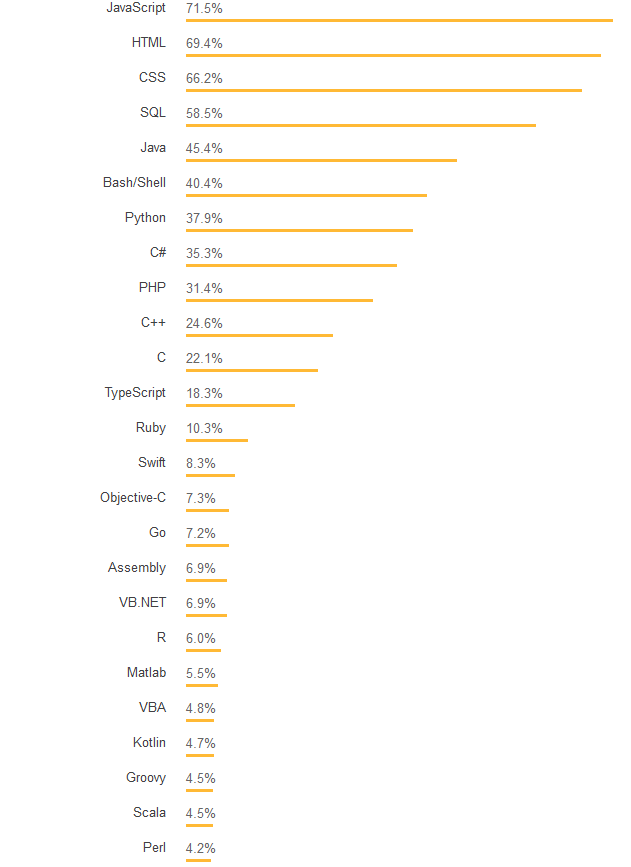
\includegraphics[width=5.00in]{images/tecnologias_populares.png}
\caption{Developer Surver Results 2018. Most popular programming, scripting and markup languagaes technologies.
 Recuperado de: https://insights.stackoverflow.com/survey/2018\#technology-\_-programming-scripting-and-markup-languages}
\label{fig:tecnologias_populares}
\end{figure}

\newpage
Además, el mismo estudio revela que Node.js es la tecnología más popular (con un 49.9\%) dentro del apartado de frameworks, librerías y herramientas:

\begin{figure}[H]
\centering
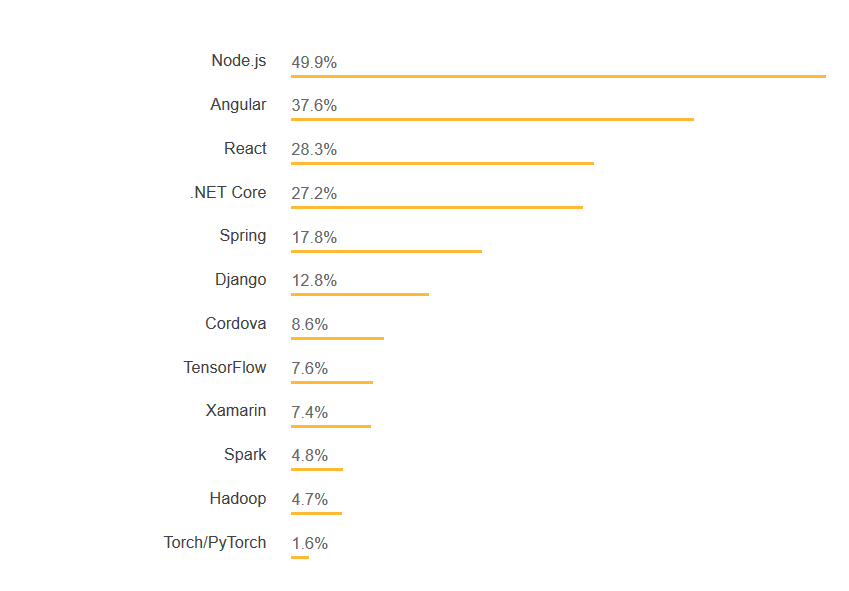
\includegraphics[width=6.00in]{images/frameworks_populares.png}
\caption{Developer Surver Results 2018. Most popular frameworks, libraries and tools. 
Recuperado de: https://insights.stackoverflow.com/survey/2018\#technology-\_-programming-scripting-and-markup-languages}
\label{fig:frameworks_populares}
\end{figure}

\lsection{Hub}
Como ya se ha explicado anteriormente, el HUB es la parte central de nuestro sistema. En él reside toda la lógica de negocio, y es el encargado
de comunicarse con la interfaz y los dispositivos.
\subsection{Tecnologías}
Para el desarrollo del HUB necesitamos utilizar tecnologías que nos permitan desarrollar un servidor REST de manera sencilla. Además, es conveniente
utilizar tecnologías modernas y mantenibles, y sobre todo, de ejecución ligera, ya que nuestro servidor se ejecutará idealmente en una raspberry.
\par
Teniendo en cuenta las necesidades tecnológicas
\subsection{Módulos}
En esta sección definiremos los módulos que nuestro HUB deberá tener y las funciones que cada uno debe cumplir. La organización por módulos, además
de permitirnos organizar nuestro software de una manera clara, nos ayudará a añadir nuevos módulos y funcionalidad el día de mañana con facilidad.
\par
Por ejemplo, en el módulo de servicios residirá toda la lógica interna, mientras que el módulo enrutador será el encargado de ``traducir`` los datos
provenientes de la red a un modelo de datos conocido e invocar a los diferentes servicios. De esta forma, si en un trabajo futuro queremos añadir
dispositivos bluetooth crearemos un módulo bluetooth que reutilice nuestros servicios.
\par
Otro ejemplo sería la migración de nuestra base de datos a otro motor diferente; sólo necesitaríamos cambiar el módulo repositorio, el resto del sistema
se mantendría intacto.
\par
Cada módulo
debe ser independiente del resto, y la modificación interna de un módulo no debería requerir la modificación del resto de módulos.
\subsection{Módulo enrutador}
Este módulo será el encargado de gestionar las conexiones entrantes y de manejar la información proveniente del exterior. Para nuestro caso, que utilizaremos
el protocolo HTTPS, en este módulo residirán las implementaciones de las APIS anteriormente definidas. Se encargará de implementar todas las rutas, encapsular
los diferentes parámetros en objetos de nuestro modelo y enviar las respuestas y códigos necesarios tras la invocación al módulo de servicios.
\subsection{Módulo middleware}
A pesar de haber separado este módulo del módulo enrutador, este módulo está totalmente ligado a la utilización del protocolo HTTPS. 
Se trata de un módulo totalmente independiente del módulo enrutador, y tendrá dos funciones principales:
\begin{itemize}
\setlength\itemsep{6pt plus 1pt minus 1pt}
\item Interceptar todas las peticiones antes de que lleguen al enrutador y validar las cabeceras y el token JWT. Si el token no es válido entonces
se envía un 401 Unauthorized sin llegar al enrutador.
\item Interceptar los errores que se provoquen durante la ejecución del programa (independientemente del módulo) y traducirlos a respuestas HTTPS. Para esto 
será necesario utilizar un modelo común de error que pueda ser interceptado por este módulo.
\end{itemize}
\subsection{Módulo de servicios}
En este módulo residirá la totalidad de nuestra lógica de negocio. A este módulo ya llegan objetos modelados con nuestro modelo de datos, y es totalmente
independiente del protocolo utilizado. Se encargará de hacer llamadas a los repositorios correspondientes y de aplicar la lógica correspondiente.
\par
Un ejemplo de lógica sería el registro de dispositivos; una vez recibido un dispositivo y sus correspondientes comandos, el servicio se encargará de hacer
las comprobaciones correspondientes y guardar el dispositivo y después sus comandos.
\par
Además, el módulo de servicios transformará los posibles errores provenientes de los repositorios para encapsularlos en errores internos. Un ejemplo sería
transformar un error \textbf{``14 SQLITE\_CANT\_OPEN``} en el siguiente error: \textbf{``Error 01: no se ha podido acceder a la base de datos sqlite``}.
\par
Tanto la entrada como la salida de datos de los métodos de nuestros servicios seguirán el modelo de datos del HUB.
\subsection{Módulo repositorio}
Este módulo contendrá toda la gestión de los datos del HUB. Será invocado por el módulo de servicios, y 
será el encargado de gestionar las conexiones con la base de datos e insertar/obtener datos de la misma.
Este módulo recibe datos modelados con nuestro modelo de datos, pero no necesariamente la manera de enviarlos/guardarlos tiene que coincidir con nuestro modelo 
de datos. Sin embargo, el retorno de los métodos de este módulo si serán datos modelados.
\par
Si en un futuro se realizasen llamadas a terceros, una API de Google por ejemplo, las llamadas a esas APIS también se realizarían desde este módulo.
\subsection{Vista general}
Por lo tanto, el diseño esquemático de la arquitectura interna del hub sería el siguiente:
\begin{figure}[H]
\centering
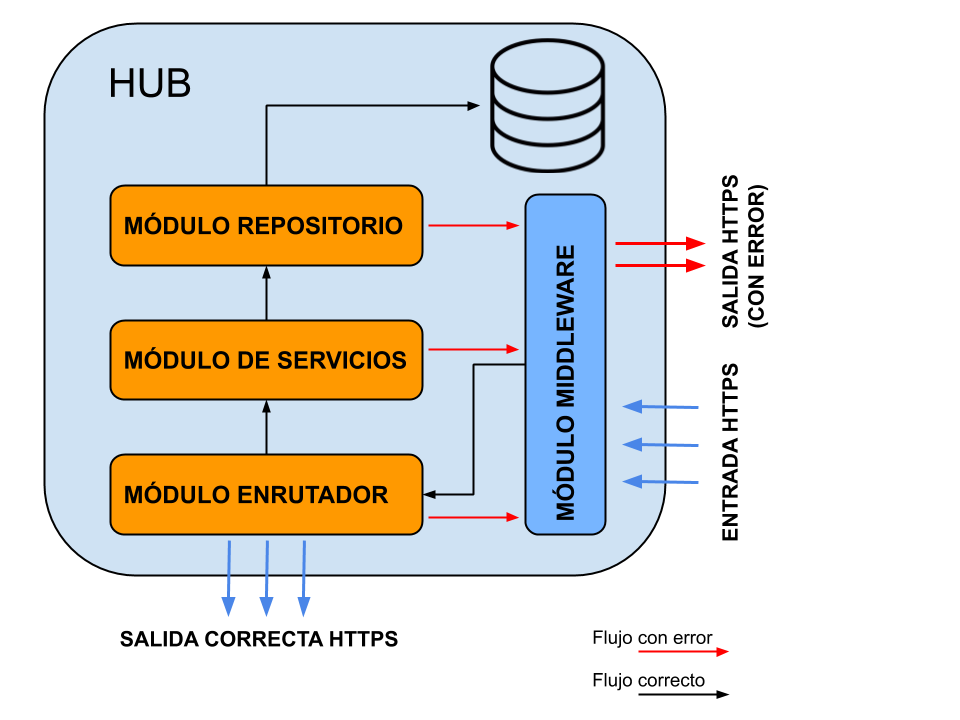
\includegraphics[width=6.00in]{images/arquitectura_hub.png}
\caption{Arquitectura interna del hub}
\label{fig:arquitectura_hub}
\end{figure}
\subsection{Configuración}
\subsection{Seguridad}
\lsection{Front end}
\subsection{Tecnologías}
\subsection{Componentes}
\subsection{Servicios}

